\chapter{Additional Information on the MPC Use Case }
\section{Statistics on Taxis in NYC}\label{appendix:sec:stats_nyc_taxis}
\subsection{Passengers per Hour}
To calculate the number of passengers per hour, one needs to estimate the number of hours during which taxis operate in New York City. The data is taken from \cite{nyc_taxi_history}. Typically, taxis operate around the clock, but for simplicity, let's assume they operate for 20 hours a day on average (accounting for downtime, maintenance, etc.). Let's first calculate the number of passengers per hour:
\[ P_{h} = \frac{1000000 \text{ passengers}}{24 \text{ hours}}\approx 41667 \]
To calculate the average number of passengers served by each taxi per hour, one can use the following formula:
\[ P/T_h = \frac{P_{h}}{T_h} \]
where $T_h = N \times s$, the number of taxis $N$ and the shift duration $s$.
Considering a 10 hours shift, i.e. $s=10$, and $N =11772$ .
\[ P/T_h = \frac{P_h}{s\times N} = \frac{ 41667}{10\times 11772} =  0.354\]
%If we consider a shift of 8 hours, the formula adjusts as follows:
%\[ P/T_h = \frac{P_h}{s\times N} = \frac{ 41,667}{8\times 11,772} =  0.442\]
\subsection{Average Passengers Carry in NYC}
Assuming each taxi operates for 10 hours total number of passengers per day to be 1000000. The average number of passengers per taxi is calculated as follows.
\[ \text{Passengers per taxi} = \frac{1000000 \text{ passengers per day}}{11772 \text{ taxis} \times 10 \text{ hours}} \approx 8.49 \text{ passengers per taxi}\]
\section{RCS Evolution}
\begin{figure}[h]
	\centering
	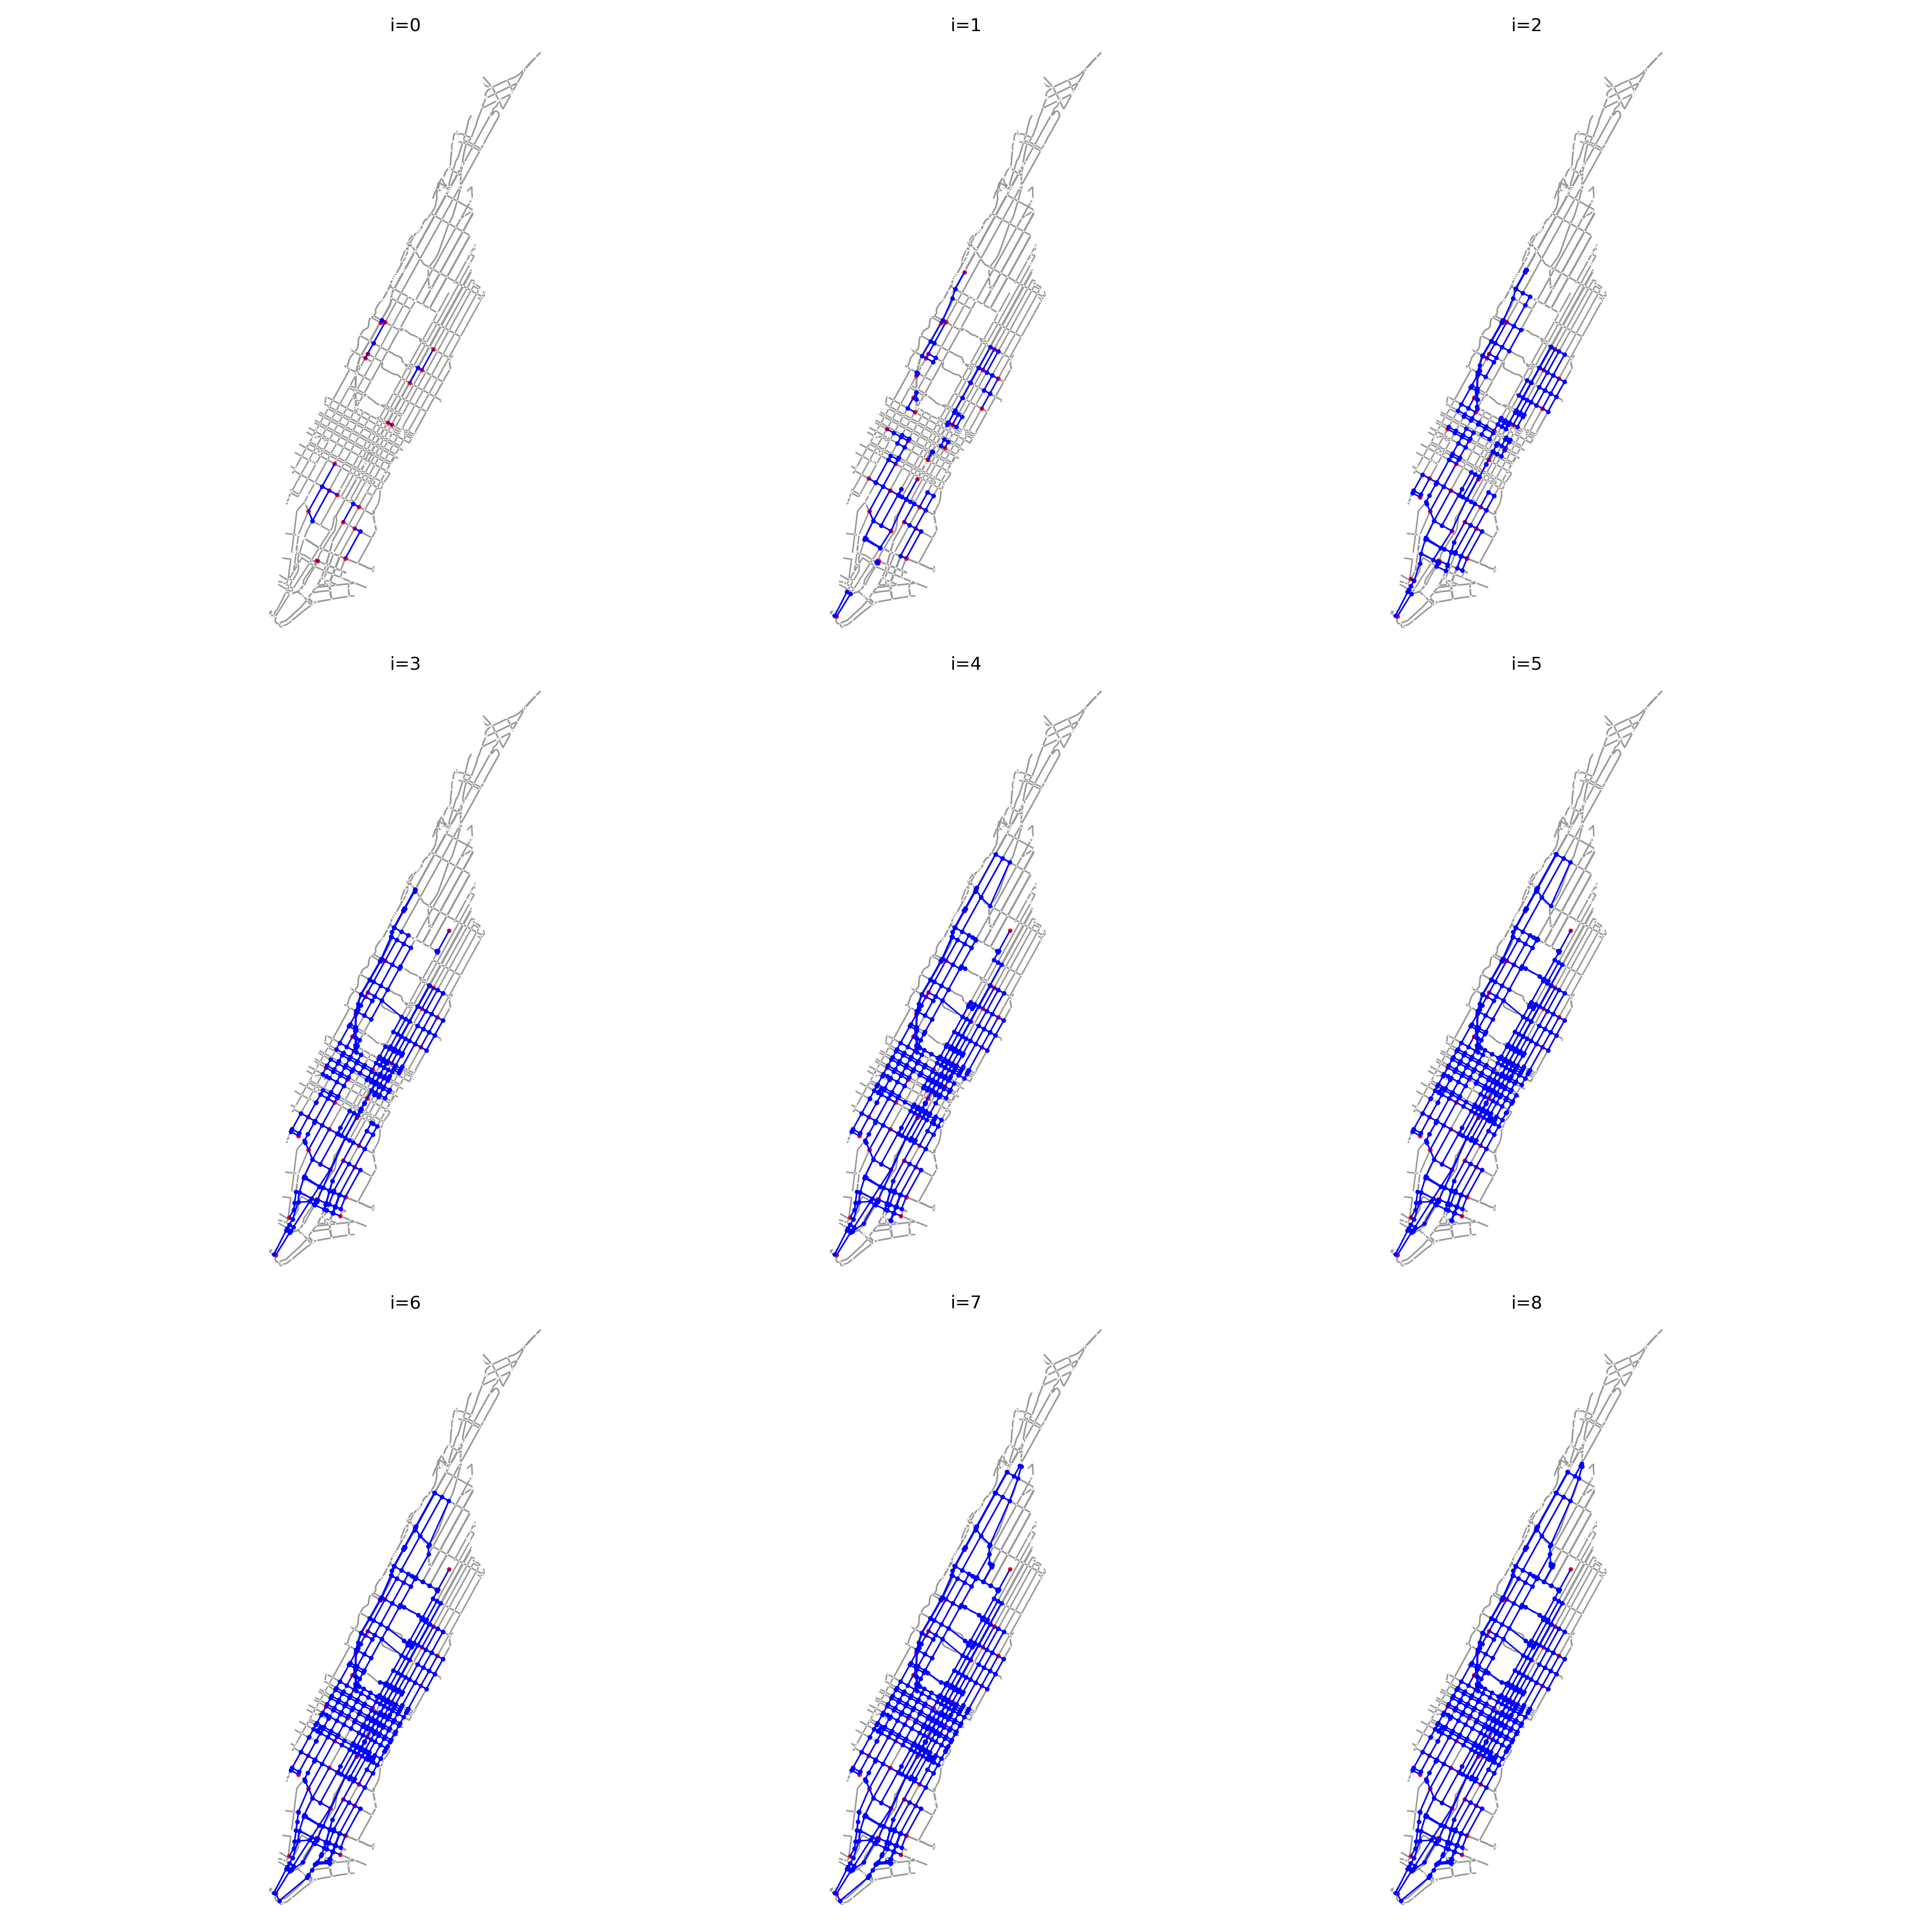
\includegraphics[width=\textwidth]{assets/img/appendix_d/evolution_nyc_plot.png}
	\caption{Depiction of The Evolution of the RCS}
	\label{app:fig:nyc_evolution}
\end{figure}